Considering the exercise's dataset, we can build the following $X$ Matrix:\\
\\
$X = \begin{Bmatrix}
	3 & 1 & 1 \\
	6.5 & 1 & 1.5\\
	5.5 & 3 & 2.5\\
	0.5 & -1 & -0.5\\
	-0.5 & 1 & 0.5
\end{Bmatrix}$\\
\\
By standardizing the matrix, we get the following $X_{std}$ matrix:\\
\\
$X_{std} = \begin{Bmatrix}
0 & 0 & 0 \\
1.28662559 & 0 & 0.5\\
0.91901828 & 1.58113883 & 1.5\\
-0.91901828 & -1.58113883 & -1.5\\
-1.28662559 & 0 &-0.5
\end{Bmatrix}$\\
\\
After standardizing the matrix, our goal is to compute the covariance matrix. We represented it as $C:$\\
\\
$C = \begin{Bmatrix}
1.25 & 0.72654774 & 1.01092011 \\
0.72654774 & 1.25 & 1.18585412\\
1.01092011 & 1.18585412 & 1.25\\
\end{Bmatrix}$\\
\\
The following step was to find the \textbf{eigenvalues} and \textbf{eigenvectors}:
\begin{verbatim}
Eigenvalues in descending order:
3.2107417718560276
0.5392582281439726
1.7237068842761345e-17

Corresponding eigenvectors:
[[-0.53316412 -0.7908806  -0.30040623]
[-0.57364312  0.59894778 -0.55874424]
[-0.62182762  0.12557641  0.77302068]]

\end{verbatim}
Also, the variance captured by each component was computed:
\begin{verbatim}
Variance captured by each component is 
[85.6197805828274, 14.380219417172604, -4.596551691403025e-16]
\end{verbatim}
Thus, we can see that PC1 has around \textbf{85\%} of contribution, while PC2 has a contribution of approximately \textbf{14\%}. With that, the dimension reduction can be started. A matrix $W$ will be created accordingly to the desired dimension.

\subsection{Reducing for 2-Dim}
The $W$ for the new 2-dimensional space:\\
\\
$W = \begin{Bmatrix}
-0.53316412 & -0.7908806\\
-0.57364312 & 0.59894778\\
-0.62182762 & 0.12557641
\end{Bmatrix}$\\
\\
By right multiplying it with $X_{std}$ we get:\\ 
\\
$X_{2-dim}$ = $X_{std}*W$ = $\begin{Bmatrix}
0 & 0\\
-0.99689641 & -0.95477901\\
-2.32973842 & 0.40855049\\
2.32973842 & -0.40855049\\
0.99689641 & 0.95477901
\end{Bmatrix}$
\\
\textbf{Graphic representation:}\\
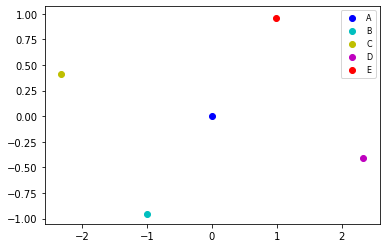
\includegraphics[scale = 0.8, width=\textwidth]{graphic2}

\subsection{Reducing for 1-Dim}
The $W$ for the new 1-dimensional space:\\
\\
$W = \begin{Bmatrix}
-0.53316412\\
-0.57364312\\
-0.62182762
\end{Bmatrix}$\\
\\
By right multiplying it with $X_{std}$ we get:\\ 
\\
$X_{1-dim}$ = $X_{std}*W$ = $\begin{Bmatrix}
0\\
-0.99689641\\
-2.32973842\\
2.32973842\\
0.99689641
\end{Bmatrix}$
\\
\textbf{Graphic representation}:
\\
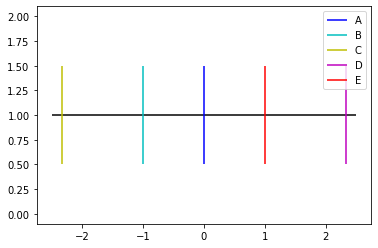
\includegraphics[scale = 0.8, width=\textwidth]{graphic1}




